% \begin{figure*}[t]
% \begin{tabular}{@{}c@{}c@{}c@{}c@{}}
% 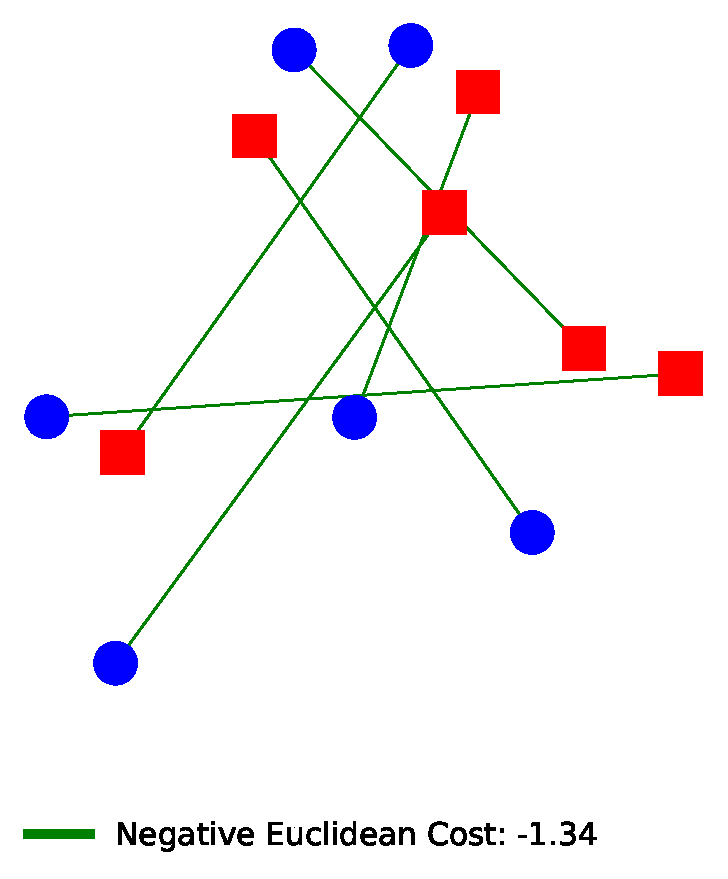
\includegraphics[width=0.25\textwidth]{figures/primal_W_1_neg_norm.pdf}&
% 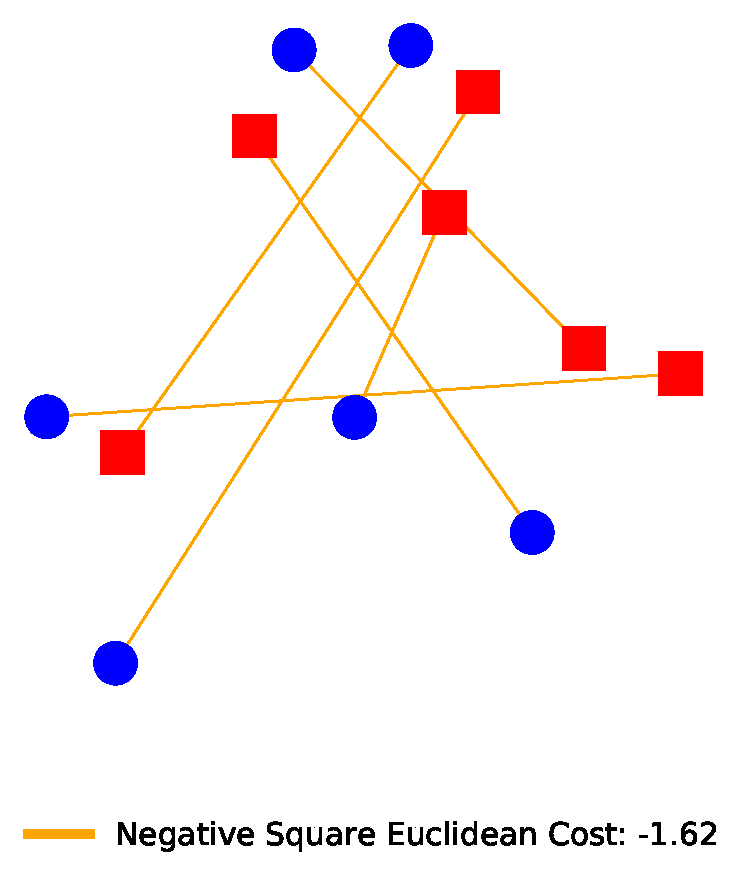
\includegraphics[width=0.25\textwidth]{figures/primal_W_2_neg_norm.pdf}&
% 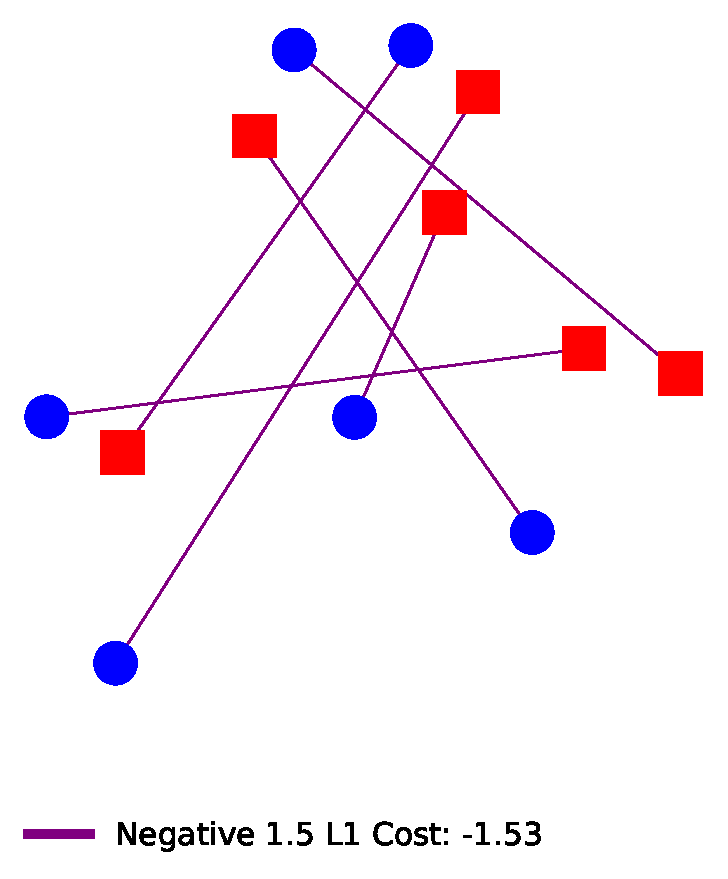
\includegraphics[width=0.25\textwidth]{figures/primal_W_3_neg_norm.pdf}&
% \includegraphics[width=0.25\textwidth]{figures/primal_W_1_2_3_neg_norm.pdf}
% % \\[-.15cm]
% % (a)&(b)&(c)&(d)
% \end{tabular}
% \caption{Comparison of the optimal matchings obtained from standard OT for three different negative costs (utilities) and $\MOT$. Blue dots and red squares represent the different type of resources available in each cake. We consider the case where there is exactly one unit of supply of each of them. \emph{Left, middle left, middle right}: Kantorovich matching between the two measures for the negative Euclidean cost, negative square Euclidean cost and negative square L1 norm respectively. These matchings represent   \emph{Right}: Equitable and optimal division of the resources given by $\MOT$. Note that the total utilities of the agents are equal and bigger than $1/N$ where $N=3$.}
% \label{fig:transport-map}
% \end{figure*}

\begin{figure}[h!]
\centering
\includegraphics[width=0.3\linewidth]{sections/appendix/aistats2021_eot/figures/primal_W_1_2_3_neg_norm.pdf}
\caption{Equitable and optimal division of the resources between $N=3$ different negative costs (i.e. utilities) given by $\MOT$. Utilities have been normalized. Blue dots and red squares represent the different elements of resources available in each cake. We consider the case where there is exactly one unit of supply per element in the cakes, which means that we consider uniform distributions. Note that the partition between the agents is equitable (i.e. utilities are equal) and proportional (i.e. utilities are larger than $1/N$).}
\label{fig:transport-map}
\end{figure}



\section{Equitable and Optimal Transport}
\label{sec:MOT}
\paragraph{Notations.} Let $\mathcal{Z}$ be a Polish space, we denote $\mathcal{M}(\mathcal{Z})$ the set of Radon measures on $\mathcal{Z}$. We call $\mathcal{M}_+(\mathcal{Z})$ the sets of positive Radon measures, and  $\mathcal{M}_+^1(\mathcal{Z})$ the set of probability measures. We denote $\mathcal{C}^b(\mathcal{Z})$ the vector space of bounded continuous functions on $\mathcal{Z}$. Let $\mathcal{X}$ and $\mathcal{Y}$ be two Polish spaces.  We denote for $\mu\in\mathcal{M}(\mathcal{X})$ and $\nu\in\mathcal{M}(\mathcal{Y})$, $\mu\otimes\nu$ the tensor product of the measures $\mu$ and $\nu$, and $\mu\ll\nu$ means that $\nu$ dominates $\mu$. We denote $\Pi_1:(x,y)\in\mathcal{X}\times\mathcal{Y}\mapsto x$ and $\Pi_2:(x,y)\in\mathcal{X}\times\mathcal{Y}\mapsto y$ respectively the projections on $\mathcal{X}$ and  $\mathcal{Y}$, which are continuous applications. For an application $g$ and a measure $\mu$, we denote $g_\sharp\mu$ the pushforward measure of $\mu$ by $g$.  For  $\mathcal{X}$ and $\mathcal{Y}$ two Polish spaces, we denote $\mathrm{LSC}(\mathcal{X}\times\mathcal{Y})$ the space of lower semi-continuous functions on $\mathcal{X}\times\mathcal{Y}$,  $\mathrm{LSC}^+(\mathcal{X}\times\mathcal{Y})$ the space of non-negative lower semi-continuous functions on $\mathcal{X}\times\mathcal{Y}$ and $\mathrm{LSC}^-_{*}(\mathcal{X}\times\mathcal{Y})$ the set of negative bounded below lower semi-continuous functions on $\mathcal{X}\times\mathcal{Y}$ . We also denote $\mathrm{C}^+(\mathcal{X}\times\mathcal{Y})$ the space of non-negative continuous functions on $\mathcal{X}\times\mathcal{Y}$ and $\mathrm{C}^-_{*}(\mathcal{X}\times\mathcal{Y})$ the set of negative continuous functions on $\mathcal{X}\times\mathcal{Y}$. Let $N\geq 1$ be an integer and denote $\Delta_N^{+}: = \{\lambda\in\mathbb{R}_+^N~\mathrm{s.t.}~\sum_{i=1}^N\lambda_i=1\}$, the probability simplex of $\mathbb{R}^N$.
% and $\Delta_N : = \{\lambda\in\mathbb{R}^N~\mathrm{s.t.}~\sum_{i=1}^N\lambda_i=1\}$. 
For two positive measures of same mass $\mu\in\mathcal{M}_+(\mathcal{X})$ and $\nu\in\mathcal{M}_+(\mathcal{Y})$, we define the set of couplings with marginals $\mu$ and $\nu$:
\begin{align*}
    \Pi_{\mu,\nu}:=\left\{\gamma~\mathrm{s.t.}~ \Pi_{1\sharp}\gamma=\mu ~,~ \Pi_{2\sharp}\gamma=\nu\right\}\; .
\end{align*}
We introduce the subset of $(\mathcal{M}_+^1(\mathcal{X})\times \mathcal{M}_+^1(\mathcal{Y}))^N$ representing marginal decomposition: 
\begin{align*}
 \textstyle\Upsilon_{\mu,\nu}^N:=&\Big\{(\mu_i,\nu_i)_{i=1}^N ~\mathrm{ s.t. }~ \sum_i \mu_i = \mu \mathrm{, } \sum_i \nu_i = \nu \\ 
 &~\mathrm{ and }~\forall i,~ \mu_i(\mathcal{X}) = \nu_i(\mathcal{Y})\;   \Big\}.
\end{align*}
We also define the following subset of $\mathcal{M}_+(\mathcal{X}\times \mathcal{Y})^N$ corresponding to the coupling decomposition:
\begin{align*}
    \Gamma^N_{\mu,\nu}:=\left\{(\gamma_i)_{i=1}^N~\mathrm{s.t.}~ \Pi_{1\sharp}\sum\gamma_i=\mu ~,~ \Pi_{2\sharp}\sum\gamma_i=\nu\right\} .
\end{align*}



\subsection{Primal Formulation}
\label{sec:primal-dual}
Consider a fair division problem where several agents aim to share two sets of resources, $\mathcal{X}$ and $\mathcal{Y}$, and assume that there is a divisible amount of each resource $x\in\mathcal{X}$ (resp. $y\in\mathcal{Y}$) that is available. Formally, we consider the case where resources are no more sets but rather distributions on these sets. Denote $\mu$ and $\nu$ the distribution of resources on respectively $\mathcal{X}$ and $\mathcal{Y}$. For example, one might think about a situation where agents want to share fruit juices and ice creams and there is a certain volume of each type of fruit juices and a certain mass of each type of ice creams available. Moreover each agent defines his or her paired preferences for each couple $(x,y)\in\mathcal{X}\times\mathcal{Y}$. Formally, each person $i$ is associated to an upper semi-continuous mapping  $u_i:\mathcal{X}\times\mathcal{Y}\xrightarrow{} \mathbb{R}^{+}$ corresponding to his or her preference for any given pair $(x,y)$. For example, one may prefer to eat chocolate ice cream with apple juice, but may prefer pineapple juice when it comes with vanilla ice cream. The total utility for an individual $i$ and a pairing $\gamma_i\in\mathcal{M}_+(\mathcal{X}\times\mathcal{Y})$ is then given by $V_i(\gamma_i) := \int u_i d\gamma_i$. To partition fairly among individuals, we maximize the minimum of individual utilities.

From a transport point of view, let assume that there are $N$ workers available to transport a distribution $\mu$ to another one $\nu$. The cost of a worker $i$ to transport a unit mass from location $x$ to the location $y$ is $c_i(x,y)$. To partition the work among the $N$ workers fairly, we minimize the maximum of individual costs. 

These problems are in fact the same where the utility $u_i$, defined in the fair division problem, might be interpreted as the opposite of the cost $c_i$ defined in the transportation problem, i.e. for all $i$, $c_i = -u_i$. The two above problem motivate the introduction of $\MOT$ defined as follows.
\begin{definition}[Equitable and Optimal Transport]
\label{def-mot}
Let $\mathcal{X}$ and $\mathcal{Y}$ be Polish spaces. Let $\mathbf{c}:=(c_i)_{1\leq i\leq N}$ be a family of bounded below lower semi-continuous cost functions on $\mathcal{X}\times \mathcal{Y}$, and $\mu\in\mathcal{M}^1_+(\mathcal{X})$ and  $\nu\in\mathcal{M}^1_+(\mathcal{Y})$. We define the equitable and optimal transport primal problem:
% \begin{align}
% \label{eq-primal}
%   \MOT_{\mathbf{c}}(\mu,\nu) :=  &\inf_{\substack{(\mu_i,\nu_i)_{i=1}^N\in\Upsilon^N_{\mu,\nu}
%         \\ \forall i,~\gamma_i\in\Pi_{\mu_i,\nu_i}}}   \max_i \int c_i d\gamma_i
% \end{align}
\begin{align}
\label{eq-primal}
\MOT_{\mathbf{c}}(\mu,\nu) := \inf_{\substack{(\gamma_i)_{i=1}^N\in\Gamma^N_{\mu,\nu}\
}}   \max_i \int c_i d\gamma_i\; .
\end{align}
\end{definition}

We prove along with Theorem~\ref{thm:duality-GOT} that the problem is well defined and the infimum is attained. Lower-semi continuity is a standard assumption in OT. In fact, it is the weakest condition to prove Kantorovich duality~\citep[Chap. 1]{villani2003topics}. Note that the problem defined here is a linear optimization problem and when $N=1$ we recover standard optimal transport. Figure~\ref{fig:transport-map} illustrates the equitable and optimal transport problem we consider. Figure~\ref{fig:transport-map-ot-view} in Appendix~\ref{appendix-illustrations} shows an illustration with respect to the transport viewpoint in the exact same setting, i.e. $c_i = - u_i$. As expected, the couplings obtained in the two situations are not the same. 
% An alternative formulation only considering coupling distributions is possible:
% \begin{align*}
%   \MOT_{\mathbf{c}}(\mu,\nu) =  &\inf_{\substack{(\gamma_i)_{i=1}^N\in\Gamma^N_{\mu,\nu}
% }}   \max_i \int c_i d\gamma_i
% \end{align*}
% In this case, the induced reparametrization is: for all $i$, $\Pi_{1\sharp}\gamma_i=\mu_i$ $\Pi_{2\sharp}\gamma_i=\nu_i$.
% Each agent $i$ receives a measure $\mu_i$ and $\nu_i$ and solves his or her optimal matching himself or herself between $\mu_i$ and $\nu_i$.
% It comes to the same thing that each agent solves its optimal matching or that the matching is made during the partition. 

We now show that in fact, $\MOT$ optimum satisfies equality constraints in case of constant sign costs, i.e. total utility/cost of each individual are equal in the optimal partition. See Appendix~\ref{prv:mot-equality} for the proof.
\begin{prop}[$\MOT$ solves the problem under equality constraints]
\label{prop:mot-equality}
Let $\mathcal{X}$ and $\mathcal{Y}$ be Polish spaces. Let $\mathbf{c}:=(c_i)_{1\leq i\leq N}\in\mathrm{LSC}^+(\mathcal{X}\times\mathcal{Y})^N\cup\mathrm{LSC}^-_{*}(\mathcal{X}\times\mathcal{Y})^N$, $\mu\in\mathcal{M}^1_+(\mathcal{X})$ and  $\nu\in\mathcal{M}^1_+(\mathcal{Y})$. Then the following are equivalent:
\vspace{-0.3cm}
\begin{itemize}
    \item $(\gamma_i^{*})_{i=1}^N\in\Gamma^N_{\mu,\nu}$ is solution of Eq.~(\ref{eq-primal}),
    \item $(\gamma_i^{*})_{i=1}^N\in \argminB\limits_{\substack{(\gamma_i)_{i=1}^N\in\Gamma^N_{\mu,\nu}
}}   \left\{t~\mathrm{s.t.}~ \forall i~\int c_i d\gamma_i=t\right\}$.
\end{itemize}
% $(\gamma_i^{*})_{i=1}^N\in\Gamma^N_{\mu,\nu}$ is solution Eq.~(\ref{eq-primal}), we have
% \begin{align*}
% \int c_i d\gamma_i^{*} = \int c_j d\gamma_j ^{*}~~\forall~i,j\in\{1,\dots,N\}\; .
% \end{align*}
\vspace{-0.4cm}
Moreover,
\vspace{-0.3cm}
\begin{align*}
  \MOT_{\mathbf{c}}(\mu,\nu) =  \min_{\substack{(\gamma_i)_{i=1}^N\in\Gamma^N_{\mu,\nu}
}}   \left\{t~\mathrm{s.t.}~ \forall i~\int c_i d\gamma_i=t\right\}\; .
\end{align*}
\end{prop}
% \begin{rmq}
% Let us now consider the case where all the cost functions are bounded non-positive lower semi-continuous functions. Then by assuming that for all $i\in\{1,\dots,N\},\exists z_i\in\mathcal{X}\times\mathcal{Y}$ s.t $$\max_{j\in\{1,\dots,N\}}\min_{z\in\mathcal{X}\times\mathcal{Y}}c_j(z)<c_i(z_i)<0$$
% then we have that
% \begin{align}
%   \MOT_{\mathbf{c}}(\mu,\nu) =  \inf_{\substack{(\mu_i,\nu_i)_{i=1}^N\in\Upsilon^N_{\mu,\nu}
%         \\ \forall i,~\gamma_i\in\Pi_{\mu_i,\nu_i}}}   \left\{t~\mathrm{s.t.}~ \forall i~\int c_i d\gamma_i=t\right\}
% \end{align}
% \end{rmq}

This property highly relies on the sign of the costs. For instance if two costs are considered, one always positive and the other always negative, then the constraints cannot be satisfied. When the cost functions are non-negatives, $\MOT$ refers to a transportation problem while when the costs are all negatives, costs become utilities and $\MOT$ refers to a fair division problem. The two points of view are concordant, but proofs and interpretations rely on the sign of the costs.

\subsection{An Equitable and Proportional Division } 
When the cost functions considered $c_i$ are all negatives, $\MOT$ become a fair division problem where the utility functions are defined as $u_i:=-c_i$. Indeed according to Proposition~\ref{prop:mot-equality}, $\MOT$ solves
\begin{align*}
\max_{\substack{(\gamma_i)_{i=1}^N\in\Gamma^N_{\mu,\nu}
}}   \left\{t~\mathrm{s.t.}~ \forall i,~\int u_i d\gamma_i=t\right\}\; .
\end{align*}
Recall that in our model, the total utility of the agent $i$ is given by $V_i(\gamma_i):=\int u_i d\gamma_i$. Therefore $\MOT$ aims to maximize the total utility of each agent $i$ while ensuring that they are all equal. Let us now analyze which fairness conditions the partition induced by $\MOT$ verifies. Assume that the utilities are normalized, i.e., $\forall i$, there exists $\gamma_i\in\mathcal{M}_+^1(\mathcal{X}\times\mathcal{Y})$ such that $V_i(\gamma_i)=1$. For example one might consider the cases where $\forall i$,  $\gamma_i=\mu\otimes\nu$ or $\gamma_i\in\argminB_{\gamma\in\Pi_{\mu,\nu}}  \int c_i d\gamma$. Then any solution $(\gamma_i^{*})_{i=1}^N\in\Gamma^N_{\mu,\nu}$ of $\MOT$ satisfies:
% These conditions
% For instance it is possible to cast the following normalization:  $V_i(\gamma^*_i)=1$ with $\gamma^*_i\in \arg\min_{\gamma\in\Pi_{\mu,\nu}}\int c_i d\gamma$. 
% Let $(\gamma_i)_{i=1}^N\in\Gamma^N_{\mu,\nu}$, we extend in a natural way the usual fairness criteria in resource allocation:
\begin{itemize}
    \item \textbf{Proportionality}: for all $i$, $V_i(\gamma_i^{*})\geq 1/N$,
    %\item \textbf{Envy-freeness}: for all $i,j$, $V_i(\gamma_i)\geq V_i(\gamma_j)$
    \item \textbf{Equitablity}: for all $i,j$, $V_i(\gamma_i^{*})=V_j(\gamma_j^{*})$.

\end{itemize}
% The intuition behind Proposition~\ref{prop:mot-equality}, some individual whose satisfaction about the allocation is strictly higher than others, will give a part of his distributions $\mu_i$ and $\nu_i$ to satisfy more of the others, but will be less satisfied. Hence this case is suboptimal and so, at the optimum, the satisfaction of individuals are the same. 
Proportionality is a standard fair division criterion for which a resource is divided among $N$ agents, giving each agent at least $1/N$ of the heterogeneous resource by his/her own subjective valuation. Therefore here, this situation corresponds to the case where the normalized utility of each agent is at least $1/N$. Moreover, an equitable division is a division of an heterogeneous resource, in which each partner is equally happy with his/her share. Here this corresponds to the case where the utility of each agent are all equal.

The problem solved by $\MOT$ is a fair division problem where heterogeneous resources have to be shared among multiple agents according to their preferences. This problem is a relaxation of the two cake-cutting problem when there are a divisible amount of each item of the cakes. In that case, cakes are distributions and $\MOT$ makes a proportional and equitable partition of them. Details are left in Appendix~\ref{prv:mot-equality}.

\paragraph{Fair Cake-cutting.} Consider the case where the cake is an heterogeneous resource and there is a certain divisible quantity of each type of resource available. For example chocolate and vanilla are two types of resource present in the cake for which a certain mass is available. In that case, each type of resource in the cake is pondered by the actual quantity present in the cake. Up to a normalization, the cake is no more the set $\mathcal{X}$ but rather a distribution on this set. Note that for the two points of view to coincide, it suffices to assume that there is exactly the same amount of mass for each type of resources available in the cake. In that case, the cake can be represented by the uniform distribution over the set $\mathcal{X}$, or equivalently the set $\mathcal{X}$ itself. When cakes are distributions, the fair cutting cake problem can be interpreted as a particular case of $\MOT$ when the utilities of the agents do not depend on the variable $y\in\mathcal{Y}$. In short, we consider that utilities are functions of the form $u_i(x,y)=v_i(x)$ for all $(x,y)\in\mathcal{X}\times\mathcal{Y}$. The normalization of utilities can be cast as follows: $\forall i$, $V_i(\mu) = \int v_i(x) d\mu(x) = 1$. Then Proposition~\ref{prop:mot-equality} shows that the partition of the cake made by $\MOT$ is proportional and equitable. Note that for $\MOT$ to coincide with the classical cake-cutting problem, one needs to consider that the uniform masses of the cake associated to each type of resource cannot be splitted. This can be interpreted as a Monge formulation~\citep{villani2003topics} of $\MOT$ which is out of the scope of this paper. 

\subsection{Optimality of $\MOT$} 
We next investigate the coupling obtained by solving $\MOT$. In the next proposition, we show that under the same assumptions of Proposition~\ref{prop:mot-equality}, $\MOT$ solutions are optimal transportation plans. See Appendix~\ref{prv:mot-otplans} for the proof.
\begin{prop}[$\MOT$ realizes optimal plans]
\label{prop:mot-otplans}
Under the same conditions of Proposition~\ref{prop:mot-equality}, for any $(\gamma_i^{*})_{i=1}^N\in\Gamma^N_{\mu,\nu}$ solution of Eq.~(\ref{eq-primal}), we have for all $i\in\{1,\dots,N\}$
\begin{equation}
  \begin{aligned}
  \label{eq-optimal-coupling}
    \gamma_i^{*}&\in\argminB_{\gamma\in\Pi_{\mu_i^{*},\nu_i^{*}}}  \int c_i d\gamma\\
    \text{where\quad} & \mu_i^{*}:=\Pi_{1\sharp}\gamma_i^{*} ~,~ \nu_i^{*}:=\Pi_{2\sharp}\gamma_i^{*}\; ,
\end{aligned}
\end{equation}
and
\begin{equation}
\begin{aligned}
\label{eq-mot-optimality}
  \MOT_{\mathbf{c}}(\mu,\nu)=  &\min_{\substack{(\mu_i,\nu_i)_{i=1}^N\in\Upsilon^N_{\mu,\nu}}} t\\
  &\mathrm{s.t.}~ \forall i~ \wass_{c_i}(\mu_i,\nu_i) =t \; .
\end{aligned}
\end{equation}
\end{prop}

Given the optimal matchings $(\gamma_i^{*})_{i=1}^N\in\Gamma^N_{\mu,\nu}$, one can easily obtain the partition of the agents of each marginals. Indeed for all $i$, $\mu_i^{*}:=\Pi_{1\sharp}\gamma_i^{*}$ and $ \nu_i^{*}:=\Pi_{2\sharp}\gamma_i^{*}$ represent respectively the portion of the agent $i$ from distributions $\mu$ and $\nu$.

\begin{rmq}[Utilitarian and Optimal Transport]
To contrast with $\MOT$, an alternative problem is to maximize the sum of the total utilities of agents, or equivalently minimize the sum of the total costs of agents. This problem can be cast as follows:
\begin{align}
\label{eq-UOT}
  \inf_{\substack{(\gamma_i)_{i=1}^N\in\Gamma^N_{\mu,\nu}\
}}  \sum_i \int c_i d\gamma_i
\end{align}
Here one aims to maximize the total utility of all the agents, while in $\MOT$ we aim to maximize the total utility per agent under egalitarian constraint. The solution of~(\ref{eq-UOT}) is not fair among agents and one can show that this problem is actually equal to $\wass_{\min_i (c_i)}(\mu,\nu)$. Details can be found in Appendix~\ref{res:min-sum}.
\end{rmq} 



% We now introduce a more general version of the standard OT problem to handle multiple costs. Given $N\geq 1$ costs, the purpose here is to minimize the global cost of transportation of a distribution towards another under the constraint that the task of transportation has to be partitioned among the costs such that each cost cannot earn more than the others. One can imagine a government wishing equity among his shippers by paying them equally. Formally the problem studied here is defined as follows.
% We propose a problem The question of the choice of the cost, e.g. Euclidean distance, square Euclidian distance or any $\ell^p$ distance ($p\geq1$), might be arbitrary and even non representative for the considered problem. In this section, we propose a problem that handles multiple costs in optimal transport by allocating the transport plan locally with regards to the different cost functions.
%In the case where $d$ is a distance on $\mathcal{X}$, we have $W_d(\mu,\nu)=\sup_{f}
% \begin{align*}
% \mathcal{F}_{(c_i)_i}:=\bigcup_{\alpha\in[0,1]}\left\{(f,g)\text{:\quad} f \oplus g\leq \min(\alpha c_1,(1-\alpha)c_2)\right\}
% \end{align*}
%We can then defined the Generalized Optimal Transport problem. }
%\subsection{A Primal-Dual Formulation}
% \todo{First introduce the minmax formulation: then explain that when replacing the max with the sum we obtain the wasserstein where the cost considered in the min of all costs locally: explain difference and interests of considering the max.}
% \todo{MOT is comprised between $W_{\min}$ and $\frac{1}{N}W_{\min}$ }
% \todo{Prove that first each $\gamma_i^{*}$ is an optimal transport plan for each $c_i$ and moreover that the $\sum\gamma_i^{*}$ is also an optimal transport plan.}
% \begin{definition}[Primal problem]
% Let $\mathcal{X}$ and $\mathcal{Y}$ be Polish spaces. Let $\mathbf{c}:=(c_i)_{1\leq i\leq N}$ be a family of nonnegative lower semi-continuous cost functions on $\mathcal{X}\times \mathcal{Y}$, and $\mu\in\mathcal{M}^1_+(\mathcal{X})$ and  $\nu\in\mathcal{M}^1_+(\mathcal{Y})$. We define the \emph{multiple cost optimal transport primal problem}:
% \begin{align}
% \label{eq-primal}
%   \MOT_{\mathbf{c}}(\mu,\nu) :=  &\inf_{(t,\gamma)\in\mathbb{R}\times\Gamma_{\mu,\nu}^N}   \hspace{0.5em} \left\{t~\mathrm{s.t.}~\forall i\in\{1,\dots,N\},\right.\\
%   &\left. ~ \int_{\mathcal{X}\times\mathcal{Y}}c_i(x,y)d\gamma_i(x,y) = t\right\}\nonumber
% \end{align}
% where  $\Gamma_{\mu,\nu}^N:=\left\{(\gamma_i)_{1\leq i\leq N}\in \mathcal{M}_+(\mathcal{X}\times \mathcal{Y})^N~\mathrm{ s.t. }~ \Pi_{1\sharp}\sum_i\gamma_i=\mu ~\mathrm{ and }~ \Pi_{2\sharp}\sum_i\gamma_i=\nu\right\}$. 
% \end{definition}


% We prove along with Theorem~\ref{thm:duality-GOT} that the problem is well defined and the infimum is attained. The well definition highly relies on the non negativity of the cost. For instance if two costs are considered, one always positive and the other always negative, then the constraints cannot be satisfied. Lower-semi continuity is a standard assumption in OT. In fact, it is the weakest condition to prove Kantorovich duality~\citep[Chap. 1]{villani2003topics}.Note that the problem defined here is a linear optimization problem and when $N=1$ we recover standard optimal transport. Figure~\ref{fig:transport-map} illustrates the multiple cost optimal transport problem we consider. The definition above can be interpreted as in the following example.

% \paragraph{Government and goods.} Assume a government can work with $N$ shippers to transport its goods $\mu$ from its stocks to stores $\nu$. To transport one unit of good from $x$ the location to $y$, each shipper $i$ proposes a price $c_i(x,y)$. Assuming that the shipper $i$ move just a fraction of the goods to some stores, and by denoting this coupling $\gamma_i$, the shipper will bill $\int c_id\gamma_i$. Therefore the government whose objective function is Problem~\eqref{eq-primal}  aims to find a partition of the work among the shippers that minimizes the total cost of transport while ensuring that shippers get equally paid.
% Therefore for a given partition of labor between the shippers $(\gamma_i)_{1\leq i\leq N}$, each shipper will bill $\int_{\mathcal{X}\times\mathcal{Y}}c_i(x,y)d\gamma_i$.
% Then the government whose objective function is Problem~\eqref{eq-primal} 
% aims to minimize the cost of transport while ensuring that he pays equally each shipper.
%Note that from the definition, the government will pay a single shipper less than if this shipper was alone on the market: in mathematical terms, it means that $\MOT_{\mathbf{c}}(\mu,\nu)\leq \min\limits_i\wass_{c_i}(\mu,\nu)$.

\begin{figure*}[t]
\begin{tabular}{@{}c@{}c@{}c@{}c@{}}
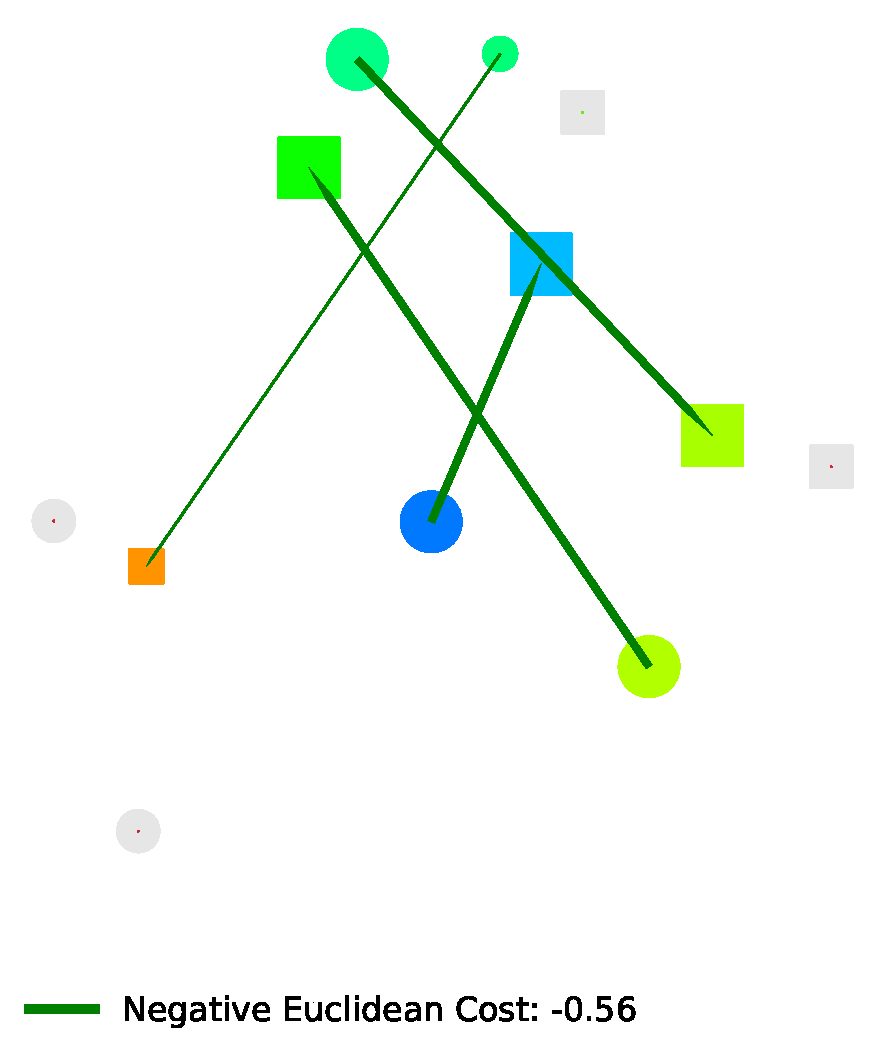
\includegraphics[width=0.24\textwidth]{sections/appendix/aistats2021_eot/figures/dual_MOT_1_neg_norm.png}&
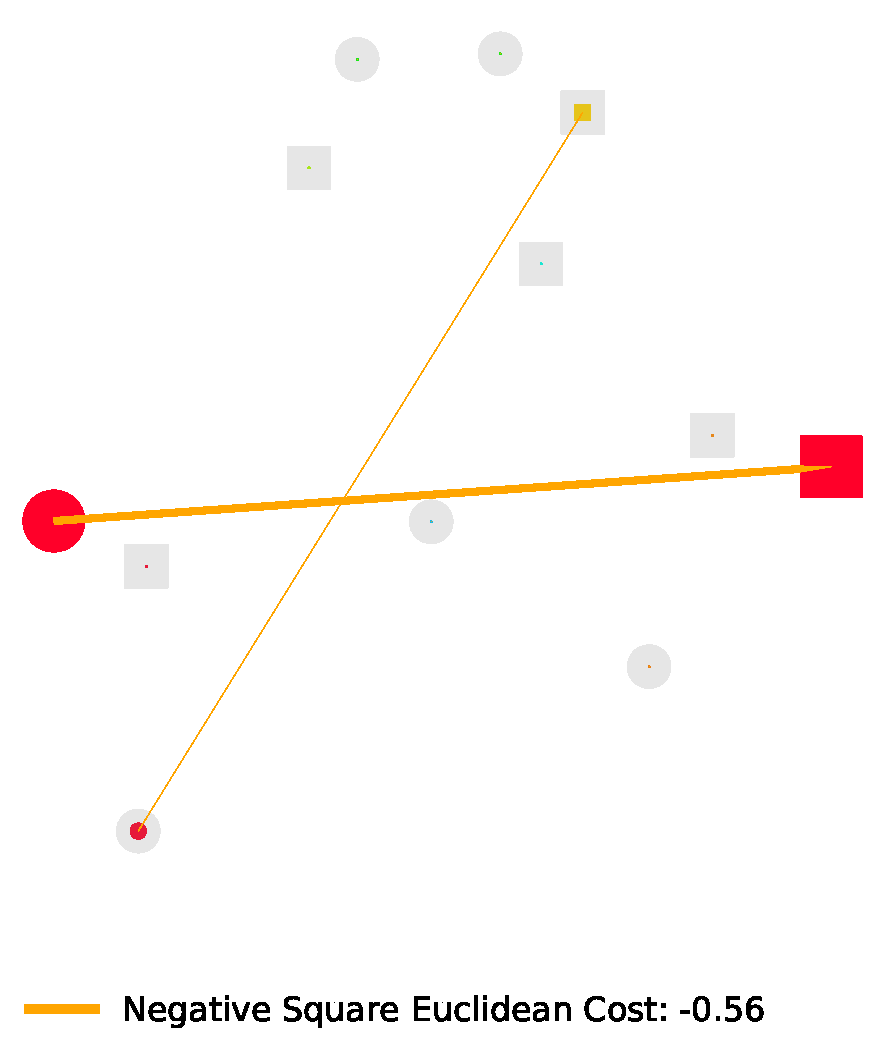
\includegraphics[width=0.24\textwidth]{sections/appendix/aistats2021_eot/figures/dual_MOT_2_neg_norm.png}&
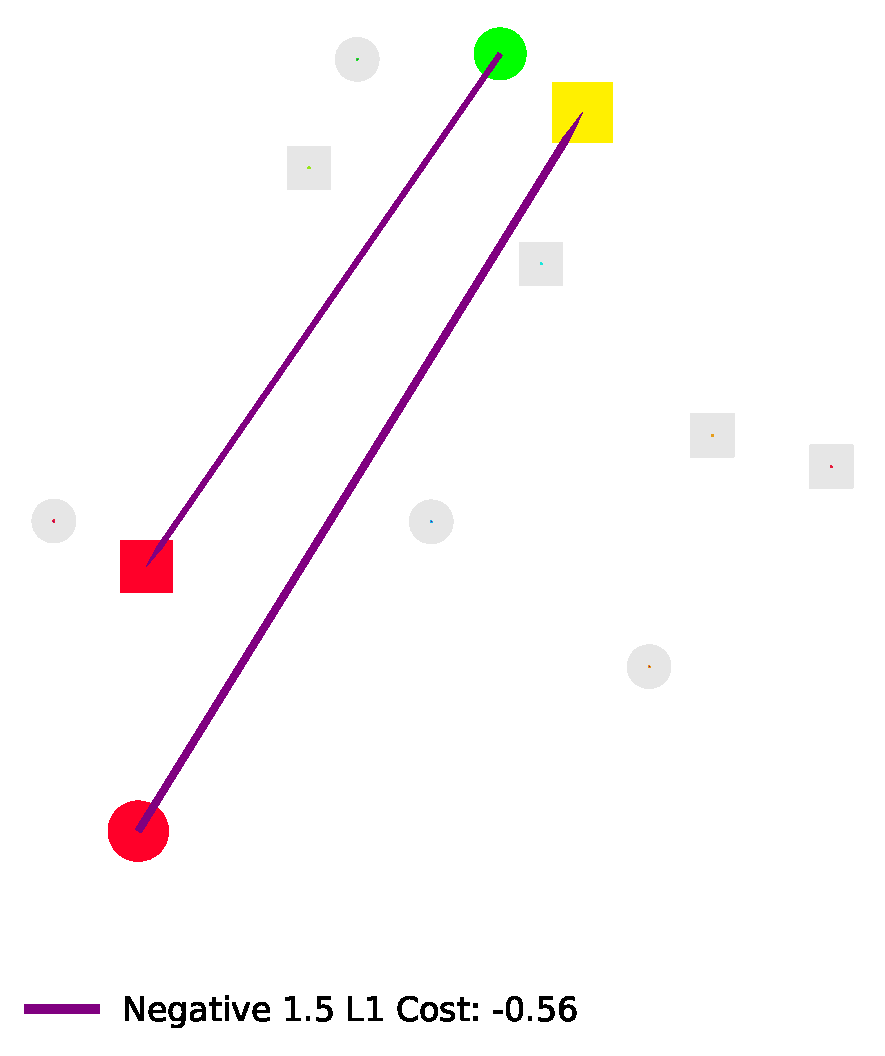
\includegraphics[width=0.24\textwidth]{sections/appendix/aistats2021_eot/figures/dual_MOT_3_neg_norm.png}&
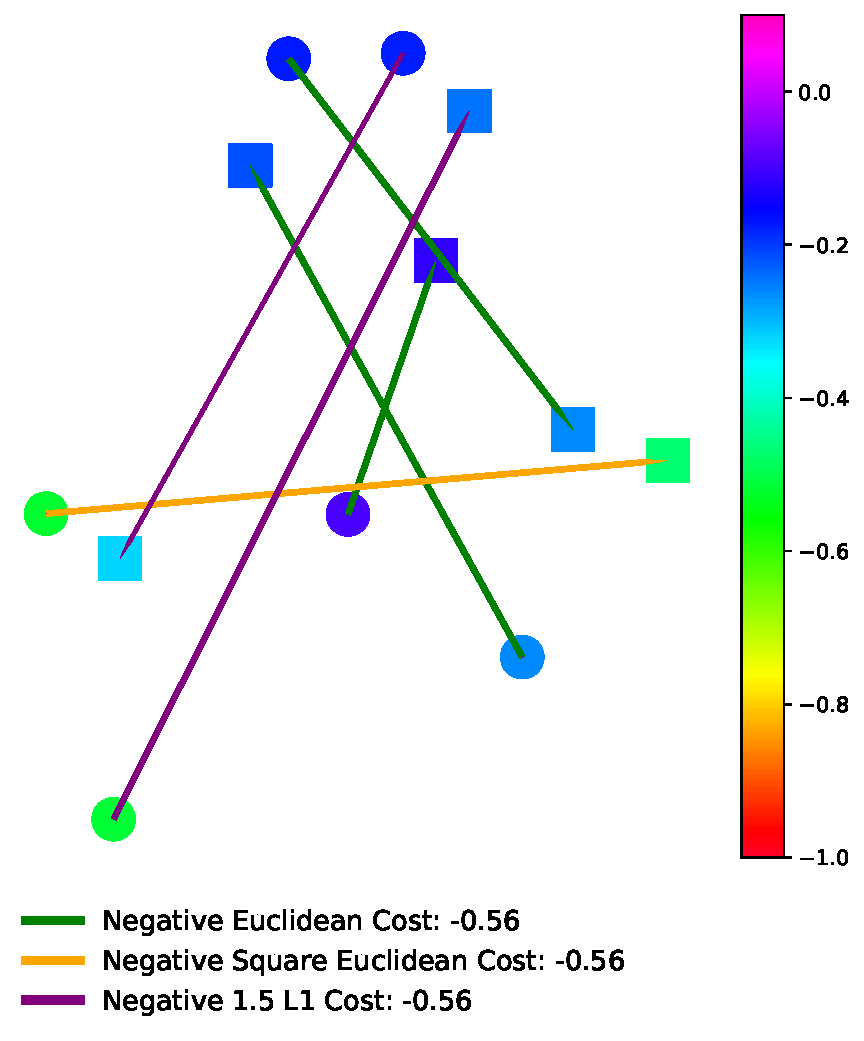
\includegraphics[width=0.275\textwidth]{sections/appendix/aistats2021_eot/figures/dual_MOT_1_2_3_neg_norm.png}
% \\[-.15cm]
% (a)&(b)&(c)&(d)
\end{tabular}
\caption{\emph{Left, middle left, middle right}: the size of dots and squares is proportional to the weight of their representing atom in the distributions $\mu_k^{*}$ and $\nu_k^{*}$ respectively. %The corresponding dual potentials $f_k^{*}$ and $g_k^{*}$ are also displayed. 
The utilities $f_k^{*}$ and $g_k^{*}$ for each point in respectively $\mu_k^{*}$ and $\nu_k^{*}$ are represented by the color of dots and squares according to the color scale on the right hand side. The gray dots and squares correspond to the points that are ignored by agent $k$ in the sense that there is no mass or almost no mass in distributions $\mu^*_k$ or $\nu^*_k$. \emph{Right}: the size of dots and squares are uniform since they correspond to the weights of uniform distributions $\mu$ and $\nu$ respectively. The values of $f^*$ and $g^*$ are given also by the color at each point. Note that each agent gets exactly the same total utility, corresponding exactly to $\MOT$. This value can be computed using dual formulation~\eqref{eq-dual} and for each figure it equals the sum of the values (encoded with colors) multiplied by the weight of each point (encoded with sizes).\label{fig:potential-dual}}
\end{figure*}


% In the following proposition we introduce a reformulation of the primal problem which allows also to consider the case where costs may be negative.
% \begin{prop}
% \label{prop:max}
% Let $\mathcal{X}$ and $\mathcal{Y}$ be Polish spaces. Let $\mathbf{c}:=(c_i)_{1\leq i\leq N}$ be a family of nonnegative lower semi-continuous costs on $\mathcal{X}\times \mathcal{Y}$, then for $\mu\in\mathcal{M}^1_+(\mathcal{X})$ and  $\nu\in\mathcal{M}^1_+(\mathcal{Y})$ we have
% \begin{align}
%     \MOT_{\mathbf{c}}(\mu,\nu):= \inf_{\gamma\in\Gamma_{\mu,\nu}^N} \max_{1\leq i\leq N}\int_{\mathcal{X}\times\mathcal{Y}}c_i(x,y)d\gamma_i(x,y)
% \end{align}
% \end{prop}
% For example in the discrete case we obtain the following linear program which does not require any assumptions on the positiviness of the costs.


% \begin{prop}[All costs contribute equally]
% \label{prop:equality}
% Let $\mathcal{X}$ and $\mathcal{Y}$ be Polish spaces. Let $\mathbf{c}:=(c_i)_{1\leq i\leq N}$ be a family of nonnegative lower semi-continuous costs on $\mathcal{X}\times \mathcal{Y}$, then for $\mu\in\mathcal{M}^1_+(\mathcal{X})$ and  $\nu\in\mathcal{M}^1_+(\mathcal{Y})$, at optimum $\gamma^*$, we have that for all  $i,j\in\{1,\dots,N\}$, $\int c_id\gamma^*_i=\int c_jd\gamma^*_j$. 
% \end{prop}
% The proof is deferred in Appendix~\ref{app:equality}. This property relies on the non negativity of the cost functions. This property is fundamental to understand the purpose of the problem we introduce. In fact, to be ``fair'' with all shippers, the government might want to equally pay them.
%The following theorem shows a strong duality result similar to standard optimal transport theory. \todo{add text}
% The next property, we prove a first duality property derived from Sion's Theorem~\citep{sion1958}, and also that infimum and supremum are attained for the considered problems. 
% \begin{prop}
% \label{prop:sup-sum-P}
% Let $\mathcal{X}$ and $\mathcal{Y}$ be Polish spaces. Let $\mathbf{c}:=(c_i)_{1\leq i\leq N}$ be a family of nonnegative lower semi-continuous costs on $\mathcal{X}\times \mathcal{Y}$, then for $\mu\in\mathcal{M}^1_+(\mathcal{X})$ and  $\nu\in\mathcal{M}^1_+(\mathcal{Y})$, we have
% \begin{align}
% \label{eq:supinf}
%     \MOT_{\mathbf{c}}(\mu,\nu)= \sup_{\lambda\in\Delta_N^{+}}\inf_{\gamma\in\Gamma^N_{\mu,\nu}} \sum_{i=1}^N\lambda_i\int_{\mathcal{X}\times\mathcal{Y}}c_i(x,y)d\gamma_i(x,y)
% \end{align}
% and both the infimum and the supremum of~\eqref{eq-primal} and~\eqref{eq:supinf} are attained. Moreover, if $\gamma^*$ be an optimum for~\eqref{eq-primal} and $\lambda^*$ an optimum for~\eqref{eq:supinf}, then $(\lambda^*,\gamma^*)$ is a saddle point for the minmax problem.
% \end{prop}
% This  rewriting is more of  theoretical purpose. If $(\lambda^*,\gamma^*)$ is an optimum for Problem~\eqref{eq:supinf}. Then, thanks to Proposition~\ref{prop:equality}, the value of $\lambda^*$ is arbitrary as long as the costs are positive and the equality of transport cost is satisfied. The following theorem shows a strong duality result similar to standard optimal transport theory.
% \todo{give interpretation for saddle point and especially $\lambda^*$ if possible}

% Assuming a government have a choice between $N$ transport shippers that propose costs $(c_1,\dots,c_N)$ to transport your goods.   you aim to partition your transport among all shippers, so that everyone works, while paying the cheapest price. Let $(\lambda^*,\gamma^*)$ be a saddle point of the problem. Then $\gamma^*_i$ represent the  transport that is allocated to shipper $i$ and $\lambda^*_i$ represent the importance given in the partition by the government to shipper $i$. Next theorem shows  strong duality holds as in standard optimal transport.

% \begin{figure*}[h!]
% \label{fig:spheres3d}\begin{tabular}{@{}c@{}c@{}c@{}}
% \includegraphics[width=0.33\textwidth]{figures/dual_W_1.pdf}&
% \includegraphics[width=0.33\textwidth]{figures/dual_W_2.pdf}&
% \includegraphics[width=0.33\textwidth]{figures/dual_W_1_2.pdf}&
% \\[-.15cm]
% (a)&(b)&(c)
% \end{tabular}
% \caption{blabla}
% \end{figure*}


% Let $\gamma^* = (\gamma^*_1,...,\gamma^*_N)$ be the optimum for the minimum problem, that exists according to next proposition. We remark for each single $i$, $\gamma^*_i$ is not a  probability distribution, but their sum is. $\gamma$ will not necessarily be fully allocated to one single coordinate. For each single $i$, $\gamma^*_i$ will represent the optimal transport plan to be locally allocated with cost $i$. The primal problem hence aims to adapt the most locally 
% ``suited'' cost $c_i$ on the ground space while being robust to ``non represntative''  costs. 

% \begin{definition}[Dual problem]
% Let $\mathcal{X}$ and $\mathcal{Y}$ be Polish spaces. Let $ \mathbf{c}=(c_i)_{1\leq i\leq N}$ be a family  of nonnegative lower semi-continuous costs on $\mathcal{X}\times \mathcal{Y}$, and $\mu\in\mathcal{M}^1_+(\mathcal{X})$ and  $\nu\in\mathcal{M}^1_+(\mathcal{Y})$. We define the \emph{generalized dual optimal transport problem}
% \begin{align*}
%     \MOT_{\mathbf{c}}(\mu,\nu):=\sup_{\lambda\in\Delta_N^{+}} \sup\limits_{(f,g)\in\mathcal{F}_{\mathbf{c}}^{\lambda}}\int_{x\in\mathcal{X}} f(x)d\mu(x)+ \int_{y\in\mathcal{Y}} g(y)d\nu(y)
% \end{align*}
% where  $\mathcal{F}^{\lambda}_{\mathbf{c}}:=\{(f,g)\in\mathcal{C}^b(\mathcal{X})\times\mathcal{C}^b(\mathcal{Y})\text{ s.t. }\forall i\in\{1,...,N\},~ f\oplus g\leq\lambda_ic_i\}.$

% \end{definition}
%This result can interpret our problem as a minimax game. 
\subsection{Dual Formulation}

Let us now introduce the dual formulation of the problem and show that strong duality holds under some mild assumptions. See Appendix~\ref{prv:duality-GOT} for the proof.
\begin{thm}[Strong Duality] 
\label{thm:duality-GOT}
Let $\mathcal{X}$ and $\mathcal{Y}$ be Polish spaces. Let $\mathbf{c}:=(c_i)_{i=1}^{N}$ be bounded below lower semi-continuous costs. Then \emph{strong duality holds}, i.e. for $(\mu,\nu)\in\mathcal{M}_{+}^{1}(\mathcal{X})\times\mathcal{M}_{+}^{1}(\mathcal{Y})$:
\begin{align}
\label{eq-dual}
   \MOT_{\mathbf{c}}(\mu,\nu)= \sup\limits_{\substack{\lambda\in\Delta^+_N\\(f,g)\in\mathcal{F}_{\mathbf{c}}^{\lambda}}}\int fd\mu+ \int gd\nu
\end{align}
where  $\mathcal{F}^{\lambda}_{\mathbf{c}}:=\{(f,g)\in\mathcal{C}^b(\mathcal{X})\times\mathcal{C}^b(\mathcal{Y})~\mathrm{ s.t. }~\forall i\in\{1,...,N\},~ f\oplus g\leq\lambda_ic_i\}$.
%and the infimum of the primal problem~(\ref{eq-primal}) is attained.
\end{thm}

This theorem holds under the same hypothesis and follows the same reasoning as the one in~\citep[Theorem 1.3]{villani2003topics}. While the primal formulation of the problem is easy to understand, we want to analyse situations where the dual variables also play a role. For that purpose we
show in the next proposition a simple characterisation
of the primal-dual optimality in case of constant sign
cost functions.  See Appendix~\ref{prv:optimality-cond} for the proof.
% The result is more difficult to interpret if we do not constraint the sign of the cost functions to be constant, but will be useful in Section~\ref{sec:entropic} to compute an efficient algorithm. 
%  a simple characterisation of the primal-dual optimality. See Appendix~\ref{appendix:optimality-condition} for the proof.
\begin{prop}
\label{prop:optimality-cond}
Let $\mathcal{X}$ and $\mathcal{Y}$ be compact Polish spaces. Let $\mathbf{c}:=(c_i)_{1\leq i\leq N}\in\mathrm{C}^+(\mathcal{X}\times\mathcal{Y})^N\cup\mathrm{C}^-_{*}(\mathcal{X}\times\mathcal{Y})^N$, $\mu\in\mathcal{M}^1_+(\mathcal{X})$ and  $\nu\in\mathcal{M}^1_+(\mathcal{Y})$. Let also $(\gamma_k)_{k=1}^N\in\Gamma^N_{\mu,\nu}$ and $(\lambda,f,g)\in\Delta_n^{+}\times\mathcal{C}^b(\mathcal{X})\times\mathcal{C}^b(\mathcal{Y})$. Then Eq.~(\ref{eq-dual}) admits a solution and the following are equivalent:
\begin{itemize}
    \item $(\gamma_k)_{k=1}^N$ is a solution of Eq.~(\ref{eq-primal}) and $(\lambda,f,g)$ is a solution of Eq.~(\ref{eq-dual}).
    \item \begin{enumerate}
        \item $\forall i\in\{1,...,N\},~ f\oplus g\leq\lambda_i c_i$
        \item $\forall i,j\in\{1,...,N\}~\int c_i d\gamma_i=\int c_j d\gamma_j$
        \item $f \oplus g= \lambda_i c_i ~~\gamma_{i}\text{-a.e.}$
    \end{enumerate}
\end{itemize}
\end{prop}
\begin{rmq}
\label{rk:lambdanonzero}
It is worth noting that when we assume that $\mathbf{c}:=(c_i)_{1\leq i\leq N}\in\mathrm{C}^+_{*}(\mathcal{X}\times\mathcal{Y})^N\cup\mathrm{C}^-_{*}(\mathcal{X}\times\mathcal{Y})^N$, then we can refine the second point of the equivalence presented in Proposition~\ref{prop:optimality-cond} by adding the following condition: $\forall i\in\{1,...,N\}~\lambda_i\neq 0$.
\end{rmq}
% To give more interpretability to this problem, we reformulate the problem as follows. Let us introduce the subset of $(\mathcal{C}^b(\mathcal{X})\times\mathcal{C}^b(\mathcal{Y}))^N$:
% $$  
% \mathcal{G}_{\mathbf{c}}^N := \left\{ (f_k,g_k)_{k=1}^N ~\mathrm{  s.t.  }~
%      \forall k,~ f_k\oplus g_k\leq c_k\right\}
%      $$

% Let us now show the  following reformulation of the problem. See Appendix~\ref{prv:dual-reformulation} for the proof.
% \begin{prop}
% \label{prop:dual-reformulation}
% Under the same assumptions of Proposition~\ref{prop:mot-equality},  we have
% \begin{align}
% \label{eq:dual_interp}
%   \MOT_{\mathbf{c}}(\mu,\nu) = & \sup\limits_{  (f_k,g_k)_{k=1}^N
%  \in\mathcal{G}^N_{\mathbf{c}}}\inf_{\substack{t\in  \mathbb{R}\\(\mu_k,\nu_k)_{k=1}^N\in\Upsilon_{\mu,\nu}^N }}
%  \hspace{0.3em}t\\
%  &\nonumber\mathrm{ s.t.}~\forall k, ~ \int f_kd\mu_k+ \int g_kd\nu_k = t 
% \end{align} 
% \end{prop}
% %By convention, the infimum equals $+\infty$ if one constraint $\int f_kd\mu_k+ \int g_kd\nu_k = t$ is not satisfied for some $k$ and equals $t$ otherwise. 


% \begin{rmq}
% As soon as  Problem~\eqref{eq-dual} admits a solution  $(\lambda^*,f^*,g^*)$ such that for all $k\in\{1,\dots,N\}$,  $\lambda^*_k\neq 0$, then by defining for all $k\in\{1,\dots,N\}$, $f_k^* = \frac{f^*}{\lambda_k^*}$ and $g_k^* = \frac{g^*}{\lambda_k^*}$, 
% % \begin{align*}
% % f_k^* = \frac{f^*}{\lambda_k^*} \text{\quad and \quad } g_k = \frac{g^*}{\lambda_k^*} 
% % \end{align*}
% the family $(f_k^{*},g_k^{*})_{k=1}^N \in\mathcal{G}^N_{\mathbf{c}}$ is an optimal solution of the Problem~\eqref{eq:dual_interp}. See Appendix~\ref{prv:dual-reformulation} for the proof.
% \end{rmq}
Given two distributions of resources represented by the measures $\mu$ and $\nu$, and $N$ utility functions denoted $(u_i)_{i=1}^N$, we want to find an \emph{equitable} and \emph{stable} partition among the agents in case of \emph{transferable utilities}. Let $k$ be an agent. We say that his or her utility is transferable when once $x\in\mathcal{X}$ and $y\in\mathcal{Y}$ get matched, he or she has to decide how to split his or her associated utility $u_k(x,y)$ . She or he divides $u_k(x,y)$ into a quantity $f_k(x)$ which can be seen as the utility of having $x$ and $g_k(y)$ for having $y$. Therefore in that problem we ask for $(\gamma_k,f_k,g_k)_{k=1}^N$ such that
\begin{align}
\label{eq-1-dual}
    u_k(x,y)=f_k(x)+g_k(y) ~~\gamma_{k}\text{-a.e.} 
\end{align}
Moreover, for the partition to be \emph{stable}~\citep{rothm}, we want to ensure that, for every agent $k$, none of the resources $x\in\mathcal{X}$ and $y\in\mathcal{Y}$ that have not been matched together for this agent would increase their utilities, $f_k(x)$ and $g_k(y)$, if there were matched together in the current matching instead. Formally we ask that for $k\in\{1,\dots,N\}$ and all $(x,y)\in\mathcal{X}\times\mathcal{Y}$,
\begin{align}
\label{eq-2-dual}
    f_k(x)+g_k(y)\geq u_k(x,y)\; .
\end{align}
Indeed if there exist $k$, $x$ and $y$ such that $u_k(x,y)>f_k(x)+g_k(y)$, then $x$ and $y$ will not be matched together in the share of the agent $k$ and he can improve his utility for both $x$ and $y$ by matching $x$ with $y$. 

Finally we aim to share equitably the resources among the agents which boils down to ask 
\begin{align}
    \label{eq-3-dual}
    \forall i,j\in\{1,...,N\}~\int u_i d\gamma_i=\int u_j d\gamma_j
\end{align}
Thanks to Proposition~\ref{prop:optimality-cond}, finding  $(\gamma_k,f_k,g_k)_{k=1}^N$ satisfying \eqref{eq-1-dual}, \eqref{eq-2-dual} and \eqref{eq-3-dual} can be done by solving Eq.~\eqref{eq-primal} and Eq.~\eqref{eq-dual}. Indeed let $(\gamma_k)_{k=1}^N$ an optimal solution of Eq.~(\ref{eq-primal}) and $(\lambda,f,g)$ an optimal solution of Eq.~(\ref{eq-dual}). Then by denoting for all $k=1,\dots,N$, 
   $f_k = \frac{f}{\lambda_k}$ and $g_k = \frac{g}{\lambda_k}$,
we obtain that $(\gamma_k,f_k,g_k)_{k=1}^N$ solves the \emph{equitable} and \emph{stable} partition problem in case of \emph{transferable utilities}. Note that again, we end up with equality constraints for the optimal dual variables. Indeed, for all $i,j\in\{1,\dots,N\}$, at optimality we have 
$\int f_i + g_i d\gamma_i = \int f_j + g_j d\gamma_j  \; $. Figure~\ref{fig:potential-dual} illustrates this formulation of the problem with dual potentials. Figure~\ref{fig:potential-dual-ot-viewpoint} in Appendix~\ref{appendix-illustrations} shows the dual solutions with respect to the transport viewpoint in the exact same setting, i.e. $c_i = - u_i$. Once again, the obtained solutions differ.



% \paragraph{Outsourcing logistics.} Assume that the government cannot solve the Linear Program~\eqref{eq-primal} stated above (primal formulation), and decides instead to outsource that task to another organization which aims making everyone work equally for the cheapest price. Assume that this organization has at disposal $N$ salespersons which may propose different prices to transport goods. Each salesperson $k$ chooses a pricing scheme with the following structure: the salesperson splits the logistic task into that of collecting and then delivering the goods, and will apply a collection price $f_k(x)$ for one unit of good located at $x$ (no matter where that unit is sent to), and a delivery price $g_k(y)$ for one unit to the location $y$ (no matter from which place that unit comes from). Then the salesperson for transporting some goods $\mu_k$ to some stores $\nu_k$ will charge $\int_{x\in\mathcal{X}} f_k(x)d\mu_k(x)+ \int_{y\in\mathcal{Y}} g_k(y)d\nu_k(y)$.

% \paragraph{Outsourcing logistics.} Assume that the government cannot solve the Linear Program~\eqref{eq-primal} stated above (primal formulation), and decides instead to outsource that task to another organization which aims making everyone work equally for the cheapest price. Assume that this organization has at disposal $N$ salespersons which may propose different prices to transport goods. Each salesperson $k$ chooses a pricing scheme with the following structure: the salesperson splits the logistic task into that of collecting and then delivering the goods, and will apply a collection price $f_k(x)$ for one unit of good located at $x$ (no matter where that unit is sent to), and a delivery price $g_k(y)$ for one unit to the location $y$ (no matter from which place that unit comes from). Then the salesperson for transporting some goods $\mu_k$ to some stores $\nu_k$ will charge $\int_{x\in\mathcal{X}} f_k(x)d\mu_k(x)+ \int_{y\in\mathcal{Y}} g_k(y)d\nu_k(y)$.


% \paragraph{Checking prices.} The government must ensure the price of transport given by the outsourcing organization will be at least lower than if he has followed the primal problem~\eqref{eq-primal}.
% For each salesperson $k$, the salesperson’s pricing scheme implies that transferring one unit of the resource from $x$ to $y$ costs exactly $f_k(x) + g_k(y)$. Yet, the government also knows that the cost of shipping one unit from $x$ to $y$ as priced by the transporting company $k$ is $c_k(x,y)$. Therefore, if for any pair $(x,y)$ the aggregate price $f_k(x) + g_k(y)$ is strictly larger that $c_k(x,y)$, the salesperson is charging more than the fair price charged by the transportation company for that task, and the government should reject the $k$-th salesperson’s offer. It is therefore in the interest of the government to check that for all pairs $(x, y)$ the prices offered by the salesperson verify $f_k\oplus g_k(x,y)\leq c_k(x,y)$. Moreover the government wants all its goods have been transported by the salespersons at their destinations. Therefore the government needs to check that $\sum_{i=1}^N \mu_i = \mu$ and that $\sum_{i=1}^N \nu_i = \nu$. Finally recall the organization wants every salesperson to earn the same, which gives for all $j,k$, $\int_{x\in\mathcal{X}} f_j(x)d\mu_j(x)+ \int_{y\in\mathcal{Y}} g_j(y)d\nu_j(y) =\int_{x\in\mathcal{X}} f_k(x)d\mu_k(x)+ \int_{y\in\mathcal{Y}} g_k(y)d\nu_k(y) $.

% \paragraph{Optimal Prices.} The salespersons must find a set of prices $(f_k,g_k)_{k=1}^N$ and a distribution of the masses $(\mu_k,\nu_k)_{k=1}^N$ that maximize their profits while minimizing the mass that they have to transport such that they earn exactly the same which is exactly the problem described in Eq.~\eqref{eq:dual_interp}. 
% \begin{rmq}[Primal-Dual Optimality]
% Note that the problem in Eq.~\eqref{eq:dual_interp} admits a saddle point as soon as
% the cost functions $(c_i)_{1\leq i\leq N}$ are continuous and the spaces $\mathcal{X}$ and $\mathcal{Y}$ are compact. Moreover at the optimum the new formulation of the problem implies that each agent receives the exact same amount of money from the government which was expected from the primal formulation. In fact, given an optimal solution of Eq.~(\ref{eq-primal}) there exists an optimal solution of Eq.~(\ref{prop:dual-reformulation}) such that for all $k\in\{1,...,N\}$ we have
% \begin{align*}
% f_k^* \oplus g_k^* (x,y) &= c_k(x,y) \mathrm{~for~all~  }(x,y)\in\mathrm{Supp}(\gamma_k^*), \\
% &\Pi_{1\sharp}\gamma_k^*=\mu_k^*,\quad\Pi_{2\sharp}\gamma_k^*=\nu_k^*.
% \end{align*} 
% Such optimal solutions can be obtained by solving Eq.~(\ref{eq-dual}).
% \end{rmq}


% \paragraph{Discrete case.} When the distributions $\mu$ and $\nu$ are discretes, primal~\eqref{eq-primal} and dual~\eqref{eq-dual} formulations
% are Linear Programs which can be solved exactly using linear solvers with complexity at least super cubic. Note that the primal problem has less constraints than the dual problems, then using primal formulation will result in a faster algorithm to compute the solution. Details on the discrete case and its dual are left in Appendix~\ref{dis:exact}.


% In case of discrete observations, we can easily adapt the problem. Let $a\in\Delta_N^{+}$ and $b\in\Delta^+_m$ and $\mathbf{C}:=(C_i)_{1\leq i\leq N}\in\left(\mathbb{R}_+^{n\times m}\right)^N$ be $N$ cost matrices. Then the discretized problem is defined as $\widehat{\MOT}_{\textbf{C}}(a,b) := \inf_{P\in\Gamma_{a,b}^N}\left\{t:~\mathrm{s.t.}~\forall i,~\langle P_i,C_i\rangle=t\right\}$ where $\Gamma_{a,b}^N:=\left\{(P_i)_{1\leq i\leq N}\in\left(\mathbb{R}_+^{n\times m}\right)^N\text{ s.t. } (\sum_i P_i)\mathbf{1}_m=a \text{ and } (\sum_i P_i^T)\mathbf{1}_n=b \right\}$. This defines a finite Linear Program whose complexity is polynomial. However, the primal problem has less constraints than the dual problem, then using primal formulation will result in a faster algorithm to compute the solution. Details on the discrete case and its dual are left in Appendix~\ref{dis:exact}.


% \subsection{Discrete Case}
% \label{sec:discrete}
% Let $a\in\Delta_N^{+}$ and $b\in\Delta_m$ and $\mathbf{C}:=(C_i)_{1\leq i\leq N}\in\left(\mathbb{R}^{n\times m}\right)^N$ be $N$ cost matrices. Let also $\mathbf{X}:=\{x_1,...,x_n\}$ and $\mathbf{Y}:=\{y_1,...,y_m\}$ two subset of $\mathcal{X}$ and $\mathcal{Y}$ respectively. Moreover we define the two following discrete measure $\mu=\sum_{i=1}^n a_i \delta_{x_i}$ and $\nu=\sum_{i=1}^n b_i \delta_{y_i}$ and for all $i$, $C_i = (c_i(x_k,y_l))_{1\leq k\leq n,1\leq l\leq m}$ where $(c_i)_{i=1}^N$ a family of cost functions. The discretized multiple cost optimal transport primal problem can be written as follows:
% \begin{align*}
% \MOT_{\mathbf{c}}(\mu,\nu)=\widehat{\MOT}_{\textbf{C}}(a,b) := \inf_{P\in\Gamma_{a,b}^N}\max_{1\leq i\leq N} \langle P_i,C_i\rangle 
% \end{align*}
% where $\Gamma_{a,b}^N:=\left\{(P_i)_{1\leq i\leq N}\in\left(\mathbb{R}_+^{n\times m}\right)^N\text{ s.t. } (\sum_i P_i)\mathbf{1}_m=a \text{ and } (\sum_i P_i^T)\mathbf{1}_n=b \right\}$. This problem can be rewritten in its Linear Programming form:
% \begin{align*}
% \widehat{\MOT}_{\mathbf{C}}(a,b)=\inf\limits_{\substack{(t,P)\in \mathbb{R}\times \Gamma_{a,b}^N\\\forall i,~ \langle P_i,C_i\rangle\leq t}} t
% \end{align*}
% As in the continuous case, strong duality holds and we can rewrite the dual in the discrete case also.
% \begin{prop}[Duality for the discrete problem]
% \label{prop:discrete-dual}

% Let $a\in\Delta_N^{+}$ and $b\in\Delta_m$ and $\mathbf{C}:=(C_i)_{1\leq i\leq N}\in\left(\mathbb{R}^{n\times m}\right)^N$ be $N$ cost matrices. Strong duality holds for the discrete problem and
% \begin{align*}
% \widehat{\MOT}_{\mathbf{C}}(a,b)=\sup_{\lambda\in\Delta_N^{+}}\sup\limits_{(f,g)\in\mathcal{F}^{\lambda}_{\mathbf{C}}} \langle f,a\rangle+\langle g,b\rangle.
% \end{align*}
% where $\mathcal{F}^{\lambda}_{\mathbf{C}}:=\{(f,g)\in\mathbb{R}_{+}^n\times\mathbb{R}_{+}^m\text{ s.t. }\forall i\in\{1,...,N\},~ f\mathbf{1}_m^T+\mathbf{1}_n g^T\leq\lambda_i C_i\}$.
% \end{prop}

% Solving Linear Programs have been widely studied in the literature, but these methods are costful since their complexity is usually polynomial. We  propose in Section~\ref{sec:entropic}  an entropic relaxation of this Linear Program to accelerate the computation.

\subsection{Link with other Probability Metrics}
\label{sec:properties}
In this section, we provide some topological properties on the object defined by the $\MOT$ problem. In particular, we make links with other known probability metrics, such as Dudley and Wasserstein metrics and give a tight upper bound. 
    
When $N=1$, recall from the definition~\eqref{eq-primal} that the problem considered is exactly the standard OT problem. Moreover any $\MOT$ problem with $k\leq N$ costs can always be rewritten as a $\MOT$ problem with $N$ costs. See Appendix~\ref{res:MOT-gene} for the proof. From this property, it is interesting to note that, for any $N\geq 1$, $\MOT$ generalizes standard Optimal Transport.
% \begin{prop} \todo{Move supp mat}
% \label{prop:sup_wasser}
% Let $\mathcal{X}$ and $\mathcal{Y}$ be Polish spaces. Let $\mathbf{c}:=(c_i)_{1\leq i\leq N}$ a family of nonnegative lower semi-continuous costs. For $(x,y)\in \mathcal{X}\times \mathcal{Y}$ and $\lambda\in\Delta_N^{+}$, we define $c_\lambda(x,y):=\min_{1\leq i\leq N}(\lambda_i c_i(x,y))$, then for any $(\mu,\nu)\in\mathcal{M}_+^{1}(\mathcal{X})\times\mathcal{M}_+^{1}(\mathcal{Y})$  
% \begin{align}
%     \MOT_{\mathbf{c}}(\mu,\nu)=\sup_{\lambda\in\Delta_N^{+}} \wass_{c_\lambda}(\mu,\nu)
% \end{align}
% \end{prop}
% This proposition and rewriting is also interpretable with regards to the choice of costs: the least informative costs will have  a weight $\lambda_i$ close to $0$, and the most informative ones  have a higher coefficient $\lambda_i$.  From the above proposition, we are able to show that as the number of cost functions increases, for well chosen costs, we recover all the $\MOT$ costs with at most the same number of costs.

% \begin{prop}
% \label{prop:gene-GOT}
% Let $\mathcal{X}$ and $\mathcal{Y}$ be Polish spaces. Let $N\geq 0$, $\mathbf{c}=(c_i)_{1\leq i\leq N}$ be a family of nonnegative lower semi-continuous costs and let us denote for all $k\in\{1,\dots,N\}$, $\mathbf{c}_k=(c_i)_{1\leq i\leq k}$. Then for all $k\in\{1,\dots,N\}$, there exists a family of costs $\mathbf{d}_k\in\text{LSC}(\mathcal{X}\times\mathcal{Y})^N$ such that  
% \begin{align}
%     \MOT_{\mathbf{d}_k}(\mu,\nu) = \MOT_{\mathbf{c}_k}(\mu,\nu)
% \end{align}
% \end{prop}
% Let us now introduce some particular cases of the $ \MOT_{\mathbf{c}}$. First we recover classical Wasserstein distance. See Appendix~\ref{prv:GOT-wass} for the proof. 
% \begin{prop}
% \label{prop:GOT-wass}
% Let $N\geq 1$, $\mathcal{X}$ and $\mathcal{Y}$ be Polish spaces and $c$ a cost function on $\mathcal{X}\times\mathcal{Y}$. Let us now define for all $i=1,\dots,N$, $c_i= N\times c$. Then for any $(\mu,\nu)\in\mathcal{M}_+^{1}(\mathcal{X})\times\mathcal{M}_+^{1}(\mathcal{Y})$  
% \begin{align}
%     \MOT_{\mathbf{c}}(\mu,\nu)=\MOT_{c}(\mu,\nu)=\wass_{c}(\mu,\nu).
% \end{align}
% \end{prop}
% In the light of interpretability we propose in Section~\ref{sec:got}, It means that if there are $N$ shippers who propose exactly the same transport cost, the the government will give them exactly the same quantity to ship and will pay them the amount of money they would get if they were alone divided by $N$. 
\paragraph{Optimal Transport.} Given a cost function $c$, if we consider the problem $\MOT$ with $N$ costs such that, for all $i$, $c_i=N\times c$ then, the problem $\MOT_\mathbf{c}$ is exactly $\wass_c$. See Appendix~\ref{res:MOT-gene} for the proof.


Now we have seen that all standard OT problems are sub-cases of the $\MOT$ problem, one may ask whether $\MOT$ can recover other families of metrics different from standard OT. Indeed we show that the $\MOT$ problem recovers an important family of $\textsc{IPM}$s with supremum taken over the space of $\alpha$-Hölder functions with $\alpha\in (0,1]$. See Appendix~\ref{prv:GOT-holder} for the proof.
\begin{prop} 
\label{prop:GOT-holder}
Let $\mathcal{X}$ be a Polish space. Let $d$ be a metric on $\mathcal{X}^2$ and $\alpha\in (0,1]$. Denote $c_1= 2\times\mathbf{1}_{x\neq y}$, $c_2=d^{\alpha}$ and $\mathbf{c}:=(c_1,(N-1)\times c_2,...,(N-1)\times c_2)\in \mathrm{LSC}(\mathcal{X}\times\mathcal{X})^N$
then for any $(\mu,\nu)\in\mathcal{M}_+^{1}(\mathcal{X})\times\mathcal{M}_+^{1}(\mathcal{X})$  
\begin{align}
\label{eq-holder}
    \MOT_{\mathbf{c}}(\mu,\nu) =\sup_{f\in B_{d^{\alpha}}(\mathcal{X})} \int_{\mathcal{X}} f d\mu - \int_{\mathcal{X}} f d\nu
\end{align}
where $B_{d^{\alpha}}(\mathcal{X}):=\left\{f\in C^{b}(\mathcal{X})\mathrm{:}~\Vert f\Vert_{\infty}+\lVert f\rVert_\alpha\leq 1 \right\}$ and $\lVert f\rVert_\alpha := \sup_{x\neq y}\frac{|f(x)-f(y)|}{d^{\alpha}(x,y)}$.
\end{prop}

\paragraph{Dudley Metric.} When $\alpha=1$, then for $(\mu,\nu)\in\mathcal{M}_+^{1}(\mathcal{X})\times\mathcal{M}_+^{1}(\mathcal{X})$, we have 
$$\MOT_{\mathbf{c}}(\mu,\nu) = \MOT_{(c_1,d)}(\mu,\nu) = \beta_d(\mu,\nu)$$
where  $\beta_d$ is the \textit{Dudley Metric}~\citep{dudley1966weak}. In other words, the Dudley metric can be interpreted as an equitable and optimal transport between the measures with the trivial cost and a metric $d$. We acknowledge that~\cite{chizat2018unbalanced} made a link between Unbalanced Optimal Transport and the ``flat metric'', an IPM close to the Dudley metric, defined on the space $\left\{f\mathrm{:}~\Vert f\Vert_{\infty}\leq 1,~\lVert f\rVert_1\leq 1 \right\}$. 

\paragraph{Weak Convergence.} When $d$ is an unbounded metric on $\mathcal{X}$, it is well known that $\wass_{d^{p}}$ with $p\in(0,+\infty)$ metrizes a convergence a bit stronger than weak convergence~\citep[Chap. 7]{villani2003topics}.  A sufficient condition for Wasserstein distances to metrize weak convergence on the space of distributions is that the metric $d$ is bounded. In contrast, metrics defined by Eq.~\eqref{eq-holder} do not require such assumptions and $\MOT_{(\mathbf{1}_{x\neq y},d^{\alpha})}$  metrizes the weak convergence of probability measures~\citep[Chap. 1-7]{villani2003topics}. 
%From an algorthmic point of view, in the case of Dudley metric,~\citep{sriperumbudur2012empirical} have reformulated the problem as a Linear Program to compute its solution, which can be recasted as our dual formulation. Using our primal formulation would make the computation faster as there are less constraints. 

For an arbitrary choice of costs $(c_i)_{1\leq i\leq N}$, we obtain a tight upper control of $\MOT$ and show how it is related to the OT problem associated to each cost involved. See Appendix~\ref{prv:ineqharmonic} for the proof. 
\begin{prop}

\label{prop:ineqharmonic}
Let  $\mathcal{X}$ and $\mathcal{Y}$ be Polish spaces. Let $\mathbf{c}:=(c_i)_{1\leq i\leq N}$ be a family of nonnegative lower semi-continuous costs. For any $(\mu,\nu)\in\mathcal{M}_+^{1}(\mathcal{X})\times\mathcal{M}_+^{1}(\mathcal{Y})$
\begin{align}
\label{eq:harmonic}
    %\frac1N  \wass_{\min\limits_i c_i}(\mu,\nu)\leq 
    \MOT_{\mathbf{c}}(\mu,\nu)\leq \left(\sum\limits_{i=1}^N\frac{1}{\wass_{c_i}(\mu,\nu)}\right)^{-1} %\leq\frac1N \min_i \wass_{c_i}(\mu,\nu)
\end{align}
\end{prop}
%To give interpretability to this inequality, one can see that the more mass the shipper $k$ carries, the more his bill increases. 
Proposition~\ref{prop:ineqharmonic} means that %the solution given by $\MOT_{\mathbf{c}}$, which is 
the minimal cost to transport all goods under the constraint that all workers contribute equally is lower than the case where agents share equitably and optimally the transport with distributions $\mu_i$ and $\nu_i$ respectively proportional to $\mu$ and $\nu$, which equals the harmonic sum written in Equation~\eqref{eq:harmonic}.

\begin{example*}
Applying the above result in the case of the  Dudley metric recovers the following inequality~\citep[Proposition 5.1]{sriperumbudur2012empirical} \begin{align*}
    \beta_d(\mu,\nu)\leq \frac{\TV(\mu,\nu)\wass_d(\mu,\nu)}{\TV(\mu,\nu)+\wass_d(\mu,\nu)}.
\end{align*}
\end{example*}
% \begin{align*}
%     \beta_d(\mu,\nu)\leq \frac{\TV(\mu,\nu)\wass_d(\mu,\nu)}{\TV(\mu,\nu)+\wass_d(\mu,\nu)} 
% \end{align*}



% \subsection{Discrete Case}
% \label{sec:discrete}
% Let $a\in\Delta_N^{+}$ and $b\in\Delta_m$ and $\mathbf{C}:=(C_i)_{1\leq i\leq N}\in\left(\mathbb{R}^{n\times m}\right)^N$ be $N$ cost matrices. Let also $\mathbf{X}:=\{x_1,...,x_n\}$ and $\mathbf{Y}:=\{y_1,...,y_m\}$ two subset of $\mathcal{X}$ and $\mathcal{Y}$ respectively. Moreover we define the two following discrete measure $\mu=\sum_{i=1}^n a_i \delta_{x_i}$ and $\nu=\sum_{i=1}^n b_i \delta_{y_i}$ and for all $i$, $C_i = (c_i(x_k,y_l))_{1\leq k\leq n,1\leq l\leq m}$ where $(c_i)_{i=1}^N$ a family of cost functions.  

% The discretized generalized primal optimal transport problem can be written as follows:
% \begin{align*}
% \MOT_{\mathbf{c}}(\mu,\nu)=\widehat{\MOT}_{\textbf{C}}(a,b) := \inf_{P\in\Gamma_{a,b}^N}\max_{1\leq i\leq N} \langle P_i,C_i\rangle 
% \end{align*}
% where $\Gamma_{a,b}^N:=\left\{(P_i)_{1\leq i\leq N}\in\left(\mathbb{R}_+^{n\times m}\right)^N\text{ s.t. } (\sum_i P_i)\mathbf{1}_m=a \text{ and } (\sum_i P_i^T)\mathbf{1}_n=b \right\}$. This problem can be rewritten in its Linear Programming form:
% \begin{align*}
% \widehat{\MOT}_{\mathbf{C}}(a,b)=\inf\limits_{\substack{(t,P)\in \mathbb{R}\times \Gamma_{a,b}^N\\\forall i,~ \langle P_i,C_i\rangle\leq t}} t
% \end{align*}
% As in the continuous case, strong duality holds and we can rewrite the dual in the discrete case also.
% \begin{prop}[Duality for the discrete problem]
% \label{prop:discrete-dual}

% Let $a\in\Delta_N^{+}$ and $b\in\Delta_m$ and $\mathbf{C}:=(C_i)_{1\leq i\leq N}\in\left(\mathbb{R}^{n\times m}\right)^N$ be $N$ cost matrices. Strong duality holds for the discrete problem and
% \begin{align*}
% \widehat{\MOT}_{\mathbf{C}}(a,b)=\sup\limits_{(f,g)\in\mathcal{F}^{\lambda}_{\mathbf{C}}} \langle f,a\rangle+\langle g,b\rangle.
% \end{align*}
% where $\mathcal{F}^{\lambda}_{\mathbf{C}}:=\{(f,g)\in\mathbb{R}_{+}^n\times\mathbb{R}_{+}^m\text{ s.t. }\forall i\in\{1,...,N\},~ f\mathbf{1}_m^T+\mathbf{1}_n g^T\leq\lambda_i C_i\}$.
% \end{prop}

% Solving Linear Programs have been widely studied in the literature, but these methods are costful since their complexity is usually polynomial. Considering the primal instead of the dual formulation may speeds up the resolution of such LP. In the particular case of the Dudley metric and classical Wasserstein distance,~\citep{sriperumbudur2012empirical} have reformulated the dual problem as a Linear Program and hence compute the solution.
% In the discrete case, it is clear that strong duality holds.
% Thanks to the duality theorem presented above, we have a simple reformulation of the primal as a linear program. Indeed the following problem 
% \begin{align}
% \MOT_{c_1,c_2}(\mu,\nu)=\inf_{(P_1,P_2)\in \Pi_{a,b}} \max\left(\langle P_1,C_1\rangle  ,\langle P_2,C_2\rangle \right)
% \end{align}
% where $C_1:=(c_1(x_i,y_j))_{i,j}$, $C_2:=(c_2(x_i,y_j))_{i,j}$ and  $$\Pi_{a,b}:=\left\{(P_1,P_2)\in\mathbb{R}_+^{n\times m}\times \mathbb{R}_+^{n\times m}\text{ s.t. } P_1\mathbf{1}+ P_2\mathbf{1}=a \text{ and } P_1^T\mathbf{1}+ P_2^T\mathbf{1}=b \right\}$$
% which can be rewritten as
% \begin{align}
% \MOT_{c_1,c_2}(\mu,\nu)=\inf_{\substack{(t,P_1,P_2)\in \mathbb{R}\times \Pi_{a,b}\\ \langle P_1,C_1\rangle\leq t\\ \langle P_2,C_2\rangle\leq t}} t
% \end{align}
% is a linear program which carries on some sense less constraint that the LP defined by the dual formulation. Indeed in the particular case of the Dudley metric, Gretton\todo{cite gretton} have reformulated the problem as a Linear Program and solve the program.


% \medskip

% Let now prove  the result holds when the spaces $\mathcal{X}$ and $\mathcal{Y}$ are not compact. We still suppose that for all $i$, $c_i$ is uniformly continuous and bounded. We denote $\Vert\mathbf{c}\rVert_\infty := \sup_i \sup_{(x,y)\in\mathcal{X}\times\mathcal{Y}} c_i(x,y)$  Let define $I^\lambda(\gamma):=\sum_i\int_{\mathcal{X}\times\mathcal{Y}}c_id\gamma_i$

% Let $\gamma^*\in \Pi^N_{\mu,\nu}$ such that $I^\lambda(\gamma^*) =\min_{\gamma_\in\Pi^N_{\mu,\nu}}I^\lambda(\gamma)$. \todo{provide existence of min}.

% Let fix $\delta\in (0,1)$. $\mathcal{X}$ and $\mathcal{Y}$ are Polish then $\exists  \mathcal{X}_0\subset \mathcal{X},  \mathcal{Y}_0\subset \mathcal{Y}$ compacts such that $\mu(\mathcal{X}_0^c) \leq  \delta$ and $\mu(\mathcal{Y}_0^c) \leq  \delta$.  It follows that $\forall i$, $\gamma^*_i((\mathcal{X}_0\times\mathcal{Y}_0)^c)\leq 2\delta$. Let define: $\gamma^{*0}$ such that for all $i$, $\gamma^{*0}_{i}=\frac{\mathbf{1}_{\mathcal{X}_0\times\mathcal{Y}_0}}{\gamma
% ^*(\mathcal{X}_0\times\mathcal{Y}_0)}\gamma^*_i$. We define $\mu_0 = \Pi_1\#\sum_i\gamma_{i}^{*0}$ and  $\nu_0 = \Pi_2\#\sum_i\gamma_{i}^{*0}$. We then naturally define $\Pi^{N}_{0,\mu_0,\nu_0} :=\left\{(\gamma_i)_{1\leq i\leq N}\in \mathcal{M}_+(\mathcal{X}_0\times \mathcal{Y}_0)^N\text{ s.t. } \Pi_1\#\sum_i\gamma_i=\mu_0 \text{ and } \Pi_2\#\sum_i\gamma_i=\nu_0\right\}$ and $I^\lambda_0(\gamma_0) := \sum_i\lambda_i\int_{\mathcal{X}_0\times\mathcal{Y}_0}c_id\gamma_{0,i}$ for $\gamma_0\in\Pi^{N}_{0,\mu_0,\nu_0}$. 

% Let $\tilde{\gamma}_0$ verifying  $I^\lambda_0(\tilde{\gamma}_0) = \min_{\gamma_0\in\Pi^N_{0,\mu_0,\nu_0}}I^\lambda_0(\gamma_0)$. Let $\tilde{\gamma} = \gamma^*(\mathcal{X}_0\times\mathcal{Y}_0)\tilde{\gamma}_0+\mathbf{1}_{(\mathcal{X}_0\times\mathcal{Y}_0)^c}\gamma^*\in \Pi^N_{\mu,\nu}$. Then we get 
% \begin{align*}
% I^\lambda(\tilde{\gamma})\leq \min_{\gamma_0\in\Pi^N_{0,\mu_0,\nu_0}}I^\lambda_0(\gamma_0)+2N\lVert \mathbf{c}\rVert_\infty\delta
% \end{align*}

% We have already proved that:

% \begin{align*}
% \sup\limits_{(f,g)\in\mathcal{F}^\lambda_{0,\mathbf{c}}}J_0^\lambda(f,g) = \inf\limits_{\gamma_0\in\Pi^N_{0,\mu_0,\nu_0}}I_0^\lambda(\gamma_0)
% \end{align*}

% with $J_0^\lambda(f,g) = \int fd\mu_0+\int gd\nu_0$ and $\mathcal{F}^\lambda_{0,\mathbf{c}}$ is the set of $(f,g)\in\mathcal{C}^b(\mathcal{X}_0)\times \mathcal{C}^b(\mathcal{Y}_0)$ satisfying, for every $i$, $f\oplus g\leq\min_i\lambda_i c_i$. Let $(\tilde{f}_0,\tilde{g}_0)\in \mathcal{F}^\lambda_\mathbf{0,c}$ such that :
% \begin{align*}
%     J_0^\lambda(\tilde{f}_0,\tilde{g}_0)\geq \sup\limits_{(f,g)\in\mathcal{F}^\lambda_{0,\mathbf{c}}}J_0^\lambda(f,g)-\delta
% \end{align*}
% Since $J_0^\lambda(0,0)=0$, we get $\sup J_0^\lambda\geq 0$ and then,  $J_0^\lambda(\tilde{f}_0,\tilde{g}_0)\geq \delta\geq-1$.For every $\gamma_0 \in \Pi^N_{0,\mu_0,\nu_0}$:

% \begin{align*}
% J_0^\lambda(\tilde{f}_0,\tilde{g}_0) = \int (\tilde{f}_0(x)+\tilde{g}_0(y))d\gamma_0(x,y)
% \end{align*}
% then we have the existence of $(x_0,y_0)\in\mathcal{X}_0\times\mathcal{Y}_0$ such that : $\tilde{f}_0(x_0)+\tilde{g}_0(y_0)\geq -1$. If we replace $(\tilde{f}_0,\tilde{g}_0)$ by $(\tilde{f}_0-s,\tilde{g}_0+s)$ for an accurate $s$, we get that: $\tilde{f}_0(x_0)\geq \frac12$
% and $\tilde{g}_0(y_0)\geq \frac12$, and then $\forall(x,y)\in\mathcal{X}_0\times\mathcal{Y}_0$:
% \begin{align*}
%     \tilde{f}_0(x)\leq c'(x,y_0)-\tilde{g}_0(y_0)\leq c'(x,y_0)+\frac12\\
%     \tilde{g}_0(y)\leq c'(x_0,y)-\tilde{f}_0(x_0)\leq c'(x_0,y)+\frac12
% \end{align*}
% where $c':=\min_i\lambda_ic_i$.  Let define $\bar{f}_0(x) = \inf_{y\in\mathcal{Y}_0}c'(x,y)-\tilde{g}_0(y)$ for $x\in\mathcal{X}$.  Then $\tilde{f}_0\leq \bar{f}_0$ on $\mathcal{X}_0$. We then get $J_0^\lambda(\bar{f}_0,\tilde{g}_0)\geq J_0^\lambda(\tilde{f}_0,\tilde{g}_0)$ and $\bar{f}_0\leq c(.,y_0)+\frac12$ on $\mathcal{X}$. Let define $\bar{g}_0(y)= \inf_{x\in\mathcal{X}}c'(x,y)-\bar{f}_0(y)$. By construction $(f_0,g_0)\in \mathcal{F}
% ^\lambda_c$ since the costs are uniformly continuous and bounded and $J_0^\lambda(\bar{f}_0,\bar{g}_0)\geq J_0^\lambda(\bar{f}_0,\tilde{g}_0)\geq J_0^\lambda(\tilde{f}_0,\tilde{g}_0)$. We also have  $\bar{g}_0\geq c(x_0,.)+\frac12$ on $\mathcal{Y}$. Then we have in particular: $\bar{g}_0\geq -\lVert\mathbf{c}\rVert-\frac12$ and $\bar{f}_0\geq -\lVert\mathbf{c}\rVert-\frac12$. Finally:

% \begin{align*}
% J(\bar{f}_0,\bar{g}_0)&=\int_{\mathcal{X}_0}\bar{f}d\mu_0+\int_{\mathcal{Y}_0}\bar{g}_0d\nu\\
% &=\sum_i\gamma_i^*(\mathcal{X}_0\times\mathcal{Y}_0)\int_{\mathcal{X}_0\times\mathcal{Y}_0}(\bar{f}_0(x)+\bar{g}_0(y))d\left(\sum_i\gamma^{*0}_i(x,y)\right)\\
% &+\int_{(\mathcal{X}_0\times\mathcal{Y}_0)^c}\bar{f}_0(x)+\bar{g}_0(y)d\left(\sum_i\gamma^{*}_i(x,y)\right)\\
% &\geq (1-2\delta)\left(\int_{\mathcal{X}_0}\bar{f}_0d\mu_0+\int_{\mathcal{Y}_0}\bar{g}_0d\nu_0\right)-(2\lVert\mathbf{c}\rVert_\infty+1)\sum_i\gamma^*((\mathcal{X}_0\times\mathcal{Y}_0)^c)\\
% &\geq (1-2\delta)J_0^\lambda(\bar{f}_0,\bar{g}_0)-2N(2\lVert\mathbf{c}\rVert_\infty+1)\delta\\
% &\geq (1-2\delta)J_0^\lambda(\tilde{f}_0,\tilde{g}_0)-2N(2\lVert\mathbf{c}\rVert_\infty+1)\delta\\
% &\geq (1-2\delta)(\inf I^\lambda_0-\delta)-2N(2\lVert\mathbf{c}\rVert_\infty+1)\delta\\
% &\geq  (1-2\delta)(\inf I^\lambda-(2N\lVert\mathbf{c}\rVert_\infty+1)\delta)-2N(2\lVert\mathbf{c}\rVert_\infty+1)\delta
% \end{align*}

% This being true for arbitrary small $\delta$, we get strong duality holds on non-compact sets $\mathcal{X}$ and $\mathcal{Y}$ 